多くのアプリケーションでは、配列はあまりわたしたちの要求を満たしてはくれません。配列を初期化する場合、どれぐらいの大きさの配列が必要かわからないからです。そのため、"動的な配列"が必要となります。Goではこのようなデータ構造を\texttt{slice}と呼びます。

\texttt{slice}は本当の意味での動的な配列ではありません。これは単なる参照型です。\texttt{slice}は常に低レイヤの\texttt{array}を指しています。\texttt{slice}の宣言も\texttt{array}と同様に長さを指定する必要はありません。

\begin{lstlisting}[numbers=none]
// arrayの宣言と同じですが、長さは必要ありません。
var fslice []int
\end{lstlisting}

次に\texttt{slice}を宣言すると同時にデータを初期化します:

\begin{lstlisting}[numbers=none]
slice := []byte {'a', 'b', 'c', 'd'}
\end{lstlisting}

\texttt{slice}はひとつの配列またはすでに存在する\texttt{slice}の中から宣言することができます。\texttt{slice}は\texttt{array[i:j]}で取得することができます。この中で\texttt{i}は配列の開始位置です。\texttt{j}は終了位置です。ただし\texttt{array[j]}は含みません。長さは\texttt{j-i}となります。

\begin{lstlisting}[numbers=none]
// 10個の要素を宣言します。要素の型はbyteの配列です。
var ar = [10]byte {'a', 'b', 'c', 'd', 'e',
                   'f', 'g', 'h', 'i', 'j'}

// byteを含む2つのsliceを宣言します
var a, b []byte

    // aポインタ配列の3つ目の要素から始まり、5つ目の要素まで
a = ar[2:5]
    //現在aの持つ要素は:ar[2]、ar[3]とar[4]です。

    // bは配列arのもう一つのsliceです。
b = ar[3:5]
// bの要素は:ar[3]とar[4]です。
\end{lstlisting}

\begin{quote}
  \texttt{slice}と配列は宣言時に区別されますのでご注意ください:配列を宣言するとき、中括弧の中で配列の長さを明示するかまたは\texttt{...}で自動的に長さを計算します。一方\texttt{slice}を宣言する時は、中括弧内には文字はありません。
\end{quote}

これらのデータ構造は以下のようになっています。

\begin{figure}[H]
  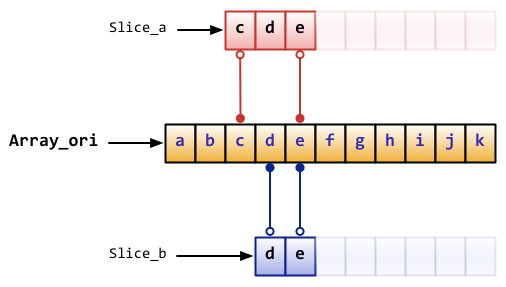
\includegraphics[width=14cm]{2.2.slice.png}
   \label{図2.3}
   \caption{sliceとarrayの対応関係図}
\end{figure}

sliceには便利な操作があります

\begin{itemize}
  \item \texttt{slice}のデフォルト開始位置は0です。\texttt{ar[:n]}などは\texttt{ar[0:n]}と等価です。
  \item \texttt{slice}の2つ目の値のデフォルトは配列の長さです。\texttt{ar[n:]}は\texttt{ar[n:len(ar)]}等価です。
  \item もし配列の中から直接\texttt{slice}を取り出す場合は、\texttt{ar[:]}というような形で指定することができます。なぜならデフォルトのはじめの値は0で2つ目は配列の長さだからです。すなわち、\texttt{ar[0:len(ar)]}と等価となります。
\end{itemize}

ここではより多くの\texttt{slice}の操作についていくつか例を挙げます:

\begin{lstlisting}[numbers=none]
// 配列を宣言
var array = [10]byte{'a', 'b', 'c', 'd', 'e',
                     'f', 'g', 'h', 'i', 'j'}
// sliceを2つ宣言
var aSlice, bSlice []byte

// 便利な操作のデモンストレーション
aSlice = array[:3] // aSlice = array[0:3] と同じ。
// aSliceには以下の要素が含まれます: a,b,c
aSlice = array[5:] // aSlice = array[5:10] と同じ。
// aSliceには以下の要素が含まれます: f,g,h,i,j
aSlice = array[:]  // aSlice = array[0:10] と同じ。
// この場合aSliceにはすべての要素が含まれます。

// sliceからsliceを取り出す
aSlice = array[3:7]  // aSliceには以下の要素が含まれます:
                     // d,e,f,g,len=4,cap=7
bSlice = aSlice[1:3] // bSlice にはaSlice[1], aSlice[2] が
// 含まれそれぞれの要素は以下のとおりです: e,f
bSlice = aSlice[:3]  // bSlice には aSlice[0], aSlice[1],
// aSlice[2] が含まれます。それぞれ以下のとおりです: d,e,f
bSlice = aSlice[0:5] // sliceのsliceに対してcapの
// 範囲内で拡張することができます。
// この時bSliceには以下の要素が含まれます:d,e,f,g,h
bSlice = aSlice[:]   // bSliceにはaSliceのすべての
                     // 要素が含まれます: d,e,f,g
\end{lstlisting}

\texttt{slice}は参照型ですので、この中の要素の値を変更すると、そのほかのすべての参照でも値が変更されます。たとえば上の\texttt{aSlice}と\texttt{bSlice}で、\texttt{aSlice}の中の要素を変更すると、\texttt{bSlice}の対応する値も同時に変更されます。

概念上では、\texttt{slice}は構造体です。この構造体には3つの要素が含まれます: 

\begin{itemize}
  \item 一つはポインタです。配列中の\texttt{slice}が示す開始位置を指しています。
  \item 長さ、つまり\texttt{slice}の長さです。
  \item 最大の長さ、\texttt{slice}の開始位置から配列の最後の位置までの長さです。
\end{itemize}


\begin{lstlisting}[numbers=none]
Array_a := [10]byte{'a', 'b', 'c', 'd', 'e', 'f', 'g', 'h', 'i', 'j'}
Slice_a := Array_a[2:5]
\end{lstlisting}

上のコードの正しい保存構造は下の図に示す通りです。

\begin{figure}[H]
  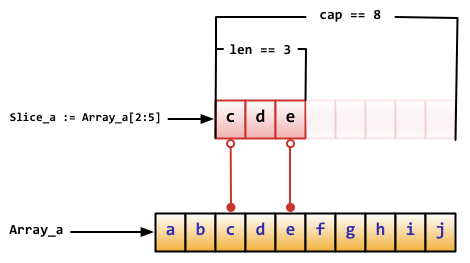
\includegraphics[width=14cm]{2.2.slice2.png}
   \label{図2.4}
   \caption{sliceに対応する配列の情報}
\end{figure}

\texttt{slice}に対しては、いくつかの便利なビルトイン関数があります:

\begin{description}
  \item[\texttt{len}] \texttt{slice}の長さを取得します。
  \item[\texttt{cap}] \texttt{slice}の最大容量を取得します。
  \item[\texttt{append}] \texttt{slice}に対して一つまたは複数の要素を追加します。その後\texttt{slice}と同じ型の\texttt{slice}を返します。
  \item[\texttt{copy}] 関数\texttt{copy}はもとの\texttt{slice}の\texttt{src}を\texttt{dst}に要素をコピーし、コピーした要素の個数を返します。
\end{description}

注:\texttt{append}関数は\texttt{slice}が参照した配列の内容を変更し得ます。そのため、参照先と同一の配列の他の\texttt{slice}にも影響します。 しかし\texttt{slice}の中に余分なスペースが無い(\texttt{(cap-len) == 0})場合、動的なメモリから新たな配列空間が割り当てられます。返される\texttt{slice}配列のポインタはこの空間を指しています。また、もとの配列の内容は変わりません。この配列を参照している他の\texttt{slice}は影響を受けません。

Go1.2より、sliceは三引数のsliceをサポートするようになりました。以前まで我々は以下のような方法でsliceまたはarrayからsliceを取り出していました

\begin{lstlisting}[numbers=none]
var array [10]int
slice := array[2:4]
\end{lstlisting}

この例ではsliceの要素数は8で、新しいバージョンでは以下のように要素数を指定することができます

\begin{lstlisting}[numbers=none]
slice = array[2:4:7]
\end{lstlisting}

上の要素数は\texttt{7-2}、即ち\texttt{5}となります。このように生成された新しいsliceでは最後の3つの要素にアクセスする方法がなくなります。

もしsliceが\texttt{array[:i:j]}のような形式だった場合は、第一引数は空と見なされ、デフォルトの0となります。


